% Options for packages loaded elsewhere
% Options for packages loaded elsewhere
\PassOptionsToPackage{unicode}{hyperref}
\PassOptionsToPackage{hyphens}{url}
%
\documentclass[
  10pt,
  ignorenonframetext,
  aspectratio=169,
]{beamer}
\newif\ifbibliography
\usepackage{pgfpages}
\setbeamertemplate{caption}[numbered]
\setbeamertemplate{caption label separator}{: }
\setbeamercolor{caption name}{fg=normal text.fg}
\beamertemplatenavigationsymbolsempty
% remove section numbering
\setbeamertemplate{part page}{
  \centering
  \begin{beamercolorbox}[sep=16pt,center]{part title}
    \usebeamerfont{part title}\insertpart\par
  \end{beamercolorbox}
}
\setbeamertemplate{section page}{
  \centering
  \begin{beamercolorbox}[sep=12pt,center]{section title}
    \usebeamerfont{section title}\insertsection\par
  \end{beamercolorbox}
}
\setbeamertemplate{subsection page}{
  \centering
  \begin{beamercolorbox}[sep=8pt,center]{subsection title}
    \usebeamerfont{subsection title}\insertsubsection\par
  \end{beamercolorbox}
}
% Prevent slide breaks in the middle of a paragraph
\widowpenalties 1 10000
\raggedbottom
\AtBeginPart{
  \frame{\partpage}
}
\AtBeginSection{
  \ifbibliography
  \else
    \frame{\sectionpage}
  \fi
}
\AtBeginSubsection{
  \frame{\subsectionpage}
}
\usepackage{iftex}
\ifPDFTeX
  \usepackage[T1]{fontenc}
  \usepackage[utf8]{inputenc}
  \usepackage{textcomp} % provide euro and other symbols
\else % if luatex or xetex
  \usepackage{unicode-math} % this also loads fontspec
  \defaultfontfeatures{Scale=MatchLowercase}
  \defaultfontfeatures[\rmfamily]{Ligatures=TeX,Scale=1}
\fi
\usepackage{lmodern}

\usetheme[]{default}
\ifPDFTeX\else
  % xetex/luatex font selection
\fi
% Use upquote if available, for straight quotes in verbatim environments
\IfFileExists{upquote.sty}{\usepackage{upquote}}{}
\IfFileExists{microtype.sty}{% use microtype if available
  \usepackage[]{microtype}
  \UseMicrotypeSet[protrusion]{basicmath} % disable protrusion for tt fonts
}{}
\makeatletter
\@ifundefined{KOMAClassName}{% if non-KOMA class
  \IfFileExists{parskip.sty}{%
    \usepackage{parskip}
  }{% else
    \setlength{\parindent}{0pt}
    \setlength{\parskip}{6pt plus 2pt minus 1pt}}
}{% if KOMA class
  \KOMAoptions{parskip=half}}
\makeatother

\usepackage{color}
\usepackage{fancyvrb}
\newcommand{\VerbBar}{|}
\newcommand{\VERB}{\Verb[commandchars=\\\{\}]}
\DefineVerbatimEnvironment{Highlighting}{Verbatim}{commandchars=\\\{\}}
% Add ',fontsize=\small' for more characters per line
\newenvironment{Shaded}{}{}
\newcommand{\AlertTok}[1]{\textcolor[rgb]{1.00,0.00,0.00}{\textbf{#1}}}
\newcommand{\AnnotationTok}[1]{\textcolor[rgb]{0.38,0.63,0.69}{\textbf{\textit{#1}}}}
\newcommand{\AttributeTok}[1]{\textcolor[rgb]{0.49,0.56,0.16}{#1}}
\newcommand{\BaseNTok}[1]{\textcolor[rgb]{0.25,0.63,0.44}{#1}}
\newcommand{\BuiltInTok}[1]{\textcolor[rgb]{0.00,0.50,0.00}{#1}}
\newcommand{\CharTok}[1]{\textcolor[rgb]{0.25,0.44,0.63}{#1}}
\newcommand{\CommentTok}[1]{\textcolor[rgb]{0.38,0.63,0.69}{\textit{#1}}}
\newcommand{\CommentVarTok}[1]{\textcolor[rgb]{0.38,0.63,0.69}{\textbf{\textit{#1}}}}
\newcommand{\ConstantTok}[1]{\textcolor[rgb]{0.53,0.00,0.00}{#1}}
\newcommand{\ControlFlowTok}[1]{\textcolor[rgb]{0.00,0.44,0.13}{\textbf{#1}}}
\newcommand{\DataTypeTok}[1]{\textcolor[rgb]{0.56,0.13,0.00}{#1}}
\newcommand{\DecValTok}[1]{\textcolor[rgb]{0.25,0.63,0.44}{#1}}
\newcommand{\DocumentationTok}[1]{\textcolor[rgb]{0.73,0.13,0.13}{\textit{#1}}}
\newcommand{\ErrorTok}[1]{\textcolor[rgb]{1.00,0.00,0.00}{\textbf{#1}}}
\newcommand{\ExtensionTok}[1]{#1}
\newcommand{\FloatTok}[1]{\textcolor[rgb]{0.25,0.63,0.44}{#1}}
\newcommand{\FunctionTok}[1]{\textcolor[rgb]{0.02,0.16,0.49}{#1}}
\newcommand{\ImportTok}[1]{\textcolor[rgb]{0.00,0.50,0.00}{\textbf{#1}}}
\newcommand{\InformationTok}[1]{\textcolor[rgb]{0.38,0.63,0.69}{\textbf{\textit{#1}}}}
\newcommand{\KeywordTok}[1]{\textcolor[rgb]{0.00,0.44,0.13}{\textbf{#1}}}
\newcommand{\NormalTok}[1]{#1}
\newcommand{\OperatorTok}[1]{\textcolor[rgb]{0.40,0.40,0.40}{#1}}
\newcommand{\OtherTok}[1]{\textcolor[rgb]{0.00,0.44,0.13}{#1}}
\newcommand{\PreprocessorTok}[1]{\textcolor[rgb]{0.74,0.48,0.00}{#1}}
\newcommand{\RegionMarkerTok}[1]{#1}
\newcommand{\SpecialCharTok}[1]{\textcolor[rgb]{0.25,0.44,0.63}{#1}}
\newcommand{\SpecialStringTok}[1]{\textcolor[rgb]{0.73,0.40,0.53}{#1}}
\newcommand{\StringTok}[1]{\textcolor[rgb]{0.25,0.44,0.63}{#1}}
\newcommand{\VariableTok}[1]{\textcolor[rgb]{0.10,0.09,0.49}{#1}}
\newcommand{\VerbatimStringTok}[1]{\textcolor[rgb]{0.25,0.44,0.63}{#1}}
\newcommand{\WarningTok}[1]{\textcolor[rgb]{0.38,0.63,0.69}{\textbf{\textit{#1}}}}

\usepackage{longtable,booktabs,array}
\usepackage{calc} % for calculating minipage widths
\usepackage{caption}
% Make caption package work with longtable
\makeatletter
\def\fnum@table{\tablename~\thetable}
\makeatother
\usepackage{graphicx}
\makeatletter
\newsavebox\pandoc@box
\newcommand*\pandocbounded[1]{% scales image to fit in text height/width
  \sbox\pandoc@box{#1}%
  \Gscale@div\@tempa{\textheight}{\dimexpr\ht\pandoc@box+\dp\pandoc@box\relax}%
  \Gscale@div\@tempb{\linewidth}{\wd\pandoc@box}%
  \ifdim\@tempb\p@<\@tempa\p@\let\@tempa\@tempb\fi% select the smaller of both
  \ifdim\@tempa\p@<\p@\scalebox{\@tempa}{\usebox\pandoc@box}%
  \else\usebox{\pandoc@box}%
  \fi%
}
% Set default figure placement to htbp
\def\fps@figure{htbp}
\makeatother





\setlength{\emergencystretch}{3em} % prevent overfull lines

\providecommand{\tightlist}{%
  \setlength{\itemsep}{0pt}\setlength{\parskip}{0pt}}



 


%%
%% Theme for BeamerClass: BHT Corporate Desgign 
%%
%% This theme bases on the theme warsaw. Beside this files, 
%% the corresponding colortheme is required:
%%    - beamercolorthemeBHT for presentations
%%
%% Usually, a beamerclass theme is split in three parts 
%% (inner, outer, color) and a theme file. These parts are
%% combined in this file.
%%
%% 28.09.2022 Beate Navarro
%%

% This program can be redistributed and/or modified under the terms
% of the GNU Public License, version 2.

\ProvidesPackage{beamerthemeBHT}[2009/04/30 V0.5 BHT beamertheme]
%%%%%%%%%%%%%%%%%%%%%%%%%%%%%%%%%%%%%%%%%%%%%%%%%%%%%%%%%
%% Presentation mode
%%
\mode<presentation>

%%%%%%%%%%%%%%%%%%%%%%%%%%%%%%%%%%%%%%%%%%%%%%%%%%%%%%%%%
%% Setting the Base
\useinnertheme[shadow=true]{rounded}
%\useoutertheme{shadow}
%\usecolortheme{BHT}
\usepackage{ifthen}
%\usepackage{minted}
\usepackage{tikz}


\setbeamerfont{block title}{size={\small}}


%\definecolor{FGtext}{RGB}{0,0,0}
\definecolor{FGtext}{RGB}{0.03, 0.27, 0.49}
\xdefinecolor{HKS51}{rgb}{0.03, 0.27, 0.49}          % HKS51, THI blau
\definecolor{THIINF}{HTML}{D7D700}          % HKS51, THI Märzrün
\definecolor{rladiesgray}{HTML}{D3D3D3}

\setbeamercolor{subtitlebar}{fg=HKS51, bg=THIINF}
\setbeamercolor*{title in head/foot}{fg=HKS51, bg=white}
\setbeamercolor*{frametitle}{fg=HKS51, bg=white}
\setbeamercolor*{framesubtitle}{fg=HKS51,bg=white}
\setbeamercolor*{frametitleLogo}{bg=white}
\setbeamercolor*{frametitleLogoDEV}{bg=HKS51!44}
\setbeamercolor*{footline}{fg=HKS51,bg=white}


\setbeamerfont*{section in head/foot}{size=\footnotesize}
\setbeamerfont*{frametitle}{size=\small}%
\setbeamerfont*{sectionnavigationhorizontal}{size=\tiny}
\setbeamerfont{section in toc}{size={\footnotesize}}
\setbeamerfont{subsection in toc}{size={\footnotesize}}

\setbeamercolor{itemize item}{fg=HKS51}
\setbeamercolor{itemize subitem}{fg=HKS51}
\setbeamercolor{itemize subsubitem}{fg=HKS51}
\setbeamertemplate{itemize items}[circle]
\setbeamercolor{enumerate item}{fg=HKS51}
\setbeamercolor{enumerate text}{fg=HKS51}

 \setbeamercolor{normal text}{fg=HKS51}
 \usebeamercolor[fg]{normal text}



%%%%%%%%%%%%%%%%%%%%%%%%%%%%%%%%%%%%%%%%%%%%%%%%%%%%%%%%%
%% Definition of the blocks
%%
\setbeamertemplate{blocks}[rounded][shadow=false]
\setbeamertemplate{section in toc}[sections numbered]
\setbeamertemplate{subsection in toc}[subsections numbered]

%%%%%%%%%%%%%%%%%%%%%%%%%%%%%%%%%%%%%%%%%%%%%%%%%%%%%%%%%
%% Setting Papersize
%%
%\setbeamersize{text margin left=2em, text margin right=2em} 

%%%%%%%%%%%%%%%%%%%%%%%%%%%%%%%%%%%%%%%%%%%%%%%%%%%%%%%%%
%% Construction of a frame's title as follows:
%% [4 squares][ frametitle               ][Logo]
%% [section navigation                         ]
%%
\newcommand{\sectionHeader}
  {
    \ifthenelse{\equal{\thesection}{0}}
      { 
        % nothing to do
      }
      {
        \ifthenelse{\equal{\thesubsection}{0}}
          {
            % section exists, subsection 0: only section in subtitlebar
            1.\thesection~ ~\insertsection
          }
          {
            % subsection existsalso: section.subsection in subtitlebar
            \thepart.\thesection.\thesubsection~--~\insertsubsection
          }
          
      }  
  }

% Subsection is a link, but needs a different color
\newcommand\disablecolorlinks{\def\HyColor@UseColor##1{}}
\makeatletter

\newcommand{\sectionHeaderLeft}
  {
    \ifthenelse{\equal{\thesection}{0}}
      {
        % nothing to do
      }
      {
	\insertsubsection      
      }
  }

\newcommand{\sectionHeaderRight}
  {
    \ifthenelse{\equal{\thesubsection}{0}}
      {
        % nothing to do
      }
      {
          \thepart.\thesection~ ~\disablecolorlinks{\insertsection}
      }
  }

\newcommand{\frameFootPart}
  {
    \ifthenelse{\equal{\thepart}{0}}
      {
        % nothing to do
      }
      {
        \hspace{1ex}\hspace{1ex}Teil \thepart:~\insertpart
      }
  }
 
\newenvironment{RMSchma}{\begin{raggedright}\itshape\doublespacing}{\end{raggedright}}

\setbeamertemplate{frametitle}
  {%
    \hspace*{-2.65em}    %% negative offset for first headerline (hack)
    \hbox{
   
      \begin{beamercolorbox}[wd=.90\paperwidth,ht=5.0ex,dp=0.5ex,left,shadow=true]{frametitle}%.618
        \usebeamerfont{frametitle}\hspace*{1.5ex}\raisebox{0.1ex}{\insertframetitle}
      \end{beamercolorbox}
     \begin{beamercolorbox}[wd=.10\paperwidth,ht=5.0ex,dp=0.5ex,center]{frametitleLogo}%
        %\usebeamerfont{section in head/foot}
        
\includegraphics[width=.04\paperwidth]{pictures/thi_logo_b_RGB}%\hspace*{2ex} 
        %
\includegraphics[width=.06\textwidth]{thi_logo_b_RGB}%\hspace*{2ex} 
      \end{beamercolorbox}%
    }
    
    \hbox{
      \begin{beamercolorbox}[wd=\paperwidth, ht=1.4ex, dp=0.5ex]{subtitlebar}
        \hspace*{0.1ex}        
                {\tiny{\sectionHeaderLeft\hfill\sectionHeaderRight}}
                \hspace*{2ex} 
      \end{beamercolorbox} 
    }
  }

% 
\setbeamertemplate{headline}[default]


%%%%%%%%%%%%%%%%%%%%%%%%%%%%%%%%%%%%%%%%%%%%%%%%%%%%%%%%%
%% Construction of a frame's footline as follows:
%% ________________________________________________
%% [ Lecture   ]           				[pages]
%%

\setbeamertemplate{footline}
   {%linie
     \color{rladiesgray}\hrule width \paperwidth depth 0pt height 0.2pt
     \vskip1pt
	% Fußzeile     
     \hbox{
       \begin{beamercolorbox}[wd=0.50\paperwidth, ht=2ex, dp=0.6ex, left]{footline}
       \hspace*{2ex} 
       \insertshorttitle
       \end{beamercolorbox}%
       \begin{beamercolorbox}[wd=0.50\paperwidth, ht=2ex, dp=0.8ex, right]{footline}
         \insertframenumber{}\,/\,\inserttotalframenumber\hspace{5ex} 
       \end{beamercolorbox}%
     }
   }



\setbeamertemplate{title page}
{%\leavevmode

  %  \begin{tikzpicture}[remember picture,overlay]
  %      %\node [xshift=0cm,yshift=0cm] at (current page.center) {
  %         \node[above right,inner sep=0pt] at (current page.south west) {
  %         % \includegraphics[width=\paperwidth, height=\paperheight]{csm_G006_VrLab_8737_b5385ff6cb}
  %         \includegraphics[width=\paperwidth]{Front}
  %      };
      \begin{tikzpicture}[remember picture,overlay]
        \node [xshift=0cm,yshift=2.3cm] at (current page.center) {
           %\node[above right,inner sep=0pt] at (current page.south west) {
           % \includegraphics[width=\paperwidth, height=\paperheight]{csm_G006_VrLab_8737_b5385ff6cb}
           \includegraphics[width=\paperwidth]{pictures/FrontBIME}
           %\includegraphics[width=0.3\textwidth]{thi_IAW_logo_wb_RGB}
        };
           
    
    % Title & Subtitle
\node
[
    above=1.5cm,
    align=left,
    fill=white!90,
    opacity=.01,
    text opacity = 1,
    inner xsep=3pt,
    inner ysep=3pt, 
    minimum width=1\textwidth,
    text width=1\textwidth
] (title) at (current page.mid east)
{
 	\LARGE    \inserttitle  \\[5pt]
	%\small \insertshorttitle \\[2pt]
    %\small \insertauthor  \\[2pt]
    \small \insertdate
};

 \end{tikzpicture}
 
}

%%%%%%%%%%%%%%%%%%%%%%%%%%%%%%%%%%%%%%%%%%%%%%%%%%%%%%%%%
%% Switches
%%

\setbeamertemplate{navigation symbols}
{}

\mode
<all>

%% Einstellung der Abstände in Table Of Contents
\makeatletter
\def\beamer@sectionintoc#1#2#3#4#5{%
  \ifnum\c@tocdepth>0%
  \ifnum#4=\beamer@showpartnumber%
  {
  \beamer@saveanother%
  \gdef\beamer@todo{}%
  \beamer@slideinframe=#1\relax%
  \expandafter\only\beamer@tocsections{\gdef\beamer@todo{%
      \beamer@tempcount=#5\relax%
      \advance\beamer@tempcount by\beamer@sectionadjust%
      \edef\inserttocsectionnumber{\the\beamer@tempcount}%
      \def\inserttocsection{\hyperlink{Navigation#3}{#2}}%
      \beamer@tocifnothide{\ifnum\c@section=#1\beamer@toc@cs\else\beamer@toc@os\fi}%
      {
        \ifbeamer@pausesections\pause\fi%
        \ifx\beamer@toc@ooss\beamer@hidetext
          \vskip0.5em
        \else
          \vskip0.3em%HIER EINSTELLEN
        \fi
        {%
          \hbox{\vbox{%
              \def\beamer@breakhere{\\}%
              \beamer@tocact{\ifnum\c@section=#1\beamer@toc@cs\else\beamer@toc@os\fi}{section in toc}}}%
         \par%
        }%
      }%
    }
  }%
  \beamer@restoreanother%
  }
  \beamer@todo%
  \fi\fi%
}
\makeatother

\renewcommand<>{\item}{\beameroriginal\item\vspace{\stretch{.2}}}

%%%%%%%%%%%%%%%%%%%%%%%%%%%%%%%%%%%%%%%%%%%%%%%%%%%%%%%%%%

\usepackage{pgfpages}

% Latin Modern: Darstellung der Schrift in PDF Dateien
\usepackage{lmodern}	

\usepackage[ngerman]{babel}
\usepackage[utf8]{inputenc}

\usepackage{graphicx}
\usepackage{longtable, tabularx}
\usepackage{multicol, multirow}
\usepackage{listings, pifont,  verbatim}
%\usepackage[thinspace]{fancyunits}
\usepackage{ifthen, xspace}
\usepackage{colortbl}
%\usepackage{mathptmx}
\usepackage{eurosym}
\usepackage{amssymb,amsmath}

\usepackage{color}
\usepackage{graphicx}


\usepackage{tcolorbox}

\usepackage{stackengine}


\usepackage{setspace}

%\setlength{\parskip}{\baselineskip} 

\usepackage[style=authortitle,backend=bibtex]{biblatex}
%\addbibresource{references.bib}

\setbeamercovered{transparent}




\usepackage{tikz}
\usetikzlibrary{tikzmark}

%\definecolor{links}{HTML}{2A1B81}
%\hypersetup{colorlinks,linkcolor=,urlcolor=links}


\newcounter{tmp}
\newcommand<>\Highlight[1]{%
\stepcounter{tmp}%
\only#2{\begin{tikzpicture}[remember picture,overlay]
\fill[green!60!black,opacity=0.5] 
  ([xshift=-.2em,yshift=2ex]pic cs:start-\thetmp)
    rectangle  
  ([xshift=.2em,yshift=-1ex]pic cs:end-\thetmp);
\end{tikzpicture}}%
\tikzmark{start-\thetmp}#1\hfill\tikzmark{end-\thetmp}%
}


\definecolor{boxgray}{RGB}{137, 148, 153}
\definecolor{boxcolor}{RGB}{244, 244, 244}
\definecolor{shadecolor}{RGB}{216, 216, 216}
\newtcolorbox{codebox}{
    colback=boxcolor,
    colframe=boxgray,
    boxrule=0.pt,
    boxsep=-2pt,
    arc=0pt}

\newtcolorbox{BHToutputbox}{
    colback=boxcolor,
    colframe=boxgray,
    boxrule=0pt,
    boxsep=-2pt,
    arc=0pt}

\newtcolorbox{blackbox}{
  colback=shadecolor,
  colframe=orange,
  coltext=black,
  boxsep=3pt,
  arc=4pt}

\newenvironment{infobox}[1]
  {
  \begin{itemize}
\setbeamertemplate{itemize item}{
    \raisebox{-.7\height}[0pt][0pt]{
      {\setkeys{Gin}{width=3em,keepaspectratio}
        \includegraphics{#1}}
    }
  }
  \setlength{\fboxsep}{1em}
  \begin{blackbox}
  \item
  }
  {
  \end{blackbox}
  \end{itemize}
  }


%\captionsetup{labelformat=empty,labelsep=none}

% highlight box
\newcommand{\highlight}[1]{%
	\colorbox{yellow!50}{$\displaystyle#1$}}


\usefonttheme[onlymath]{serif}

\AtBeginPart{}
\AtBeginSection{}
\AtBeginSubsection{}
\AtBeginSubsubsection{}
\setlength{\emergencystretch}{0em}
%\setlength{\parskip}{0pt}
\setlength{\parskip}{1.5ex plus0.5ex minus0.5ex}
\setbeamertemplate{itemize/enumerate body end}{\vspace{.6\baselineskip}} % So I'm less inclined to use \medskip and \bigskip in Markdown.


\makeatletter
\@ifpackageloaded{caption}{}{\usepackage{caption}}
\AtBeginDocument{%
\ifdefined\contentsname
  \renewcommand*\contentsname{Table of contents}
\else
  \newcommand\contentsname{Table of contents}
\fi
\ifdefined\listfigurename
  \renewcommand*\listfigurename{List of Figures}
\else
  \newcommand\listfigurename{List of Figures}
\fi
\ifdefined\listtablename
  \renewcommand*\listtablename{List of Tables}
\else
  \newcommand\listtablename{List of Tables}
\fi
\ifdefined\figurename
  \renewcommand*\figurename{Figure}
\else
  \newcommand\figurename{Figure}
\fi
\ifdefined\tablename
  \renewcommand*\tablename{Table}
\else
  \newcommand\tablename{Table}
\fi
}
\@ifpackageloaded{float}{}{\usepackage{float}}
\floatstyle{ruled}
\@ifundefined{c@chapter}{\newfloat{codelisting}{h}{lop}}{\newfloat{codelisting}{h}{lop}[chapter]}
\floatname{codelisting}{Listing}
\newcommand*\listoflistings{\listof{codelisting}{List of Listings}}
\makeatother
\makeatletter
\makeatother
\makeatletter
\@ifpackageloaded{caption}{}{\usepackage{caption}}
\@ifpackageloaded{subcaption}{}{\usepackage{subcaption}}
\makeatother

\usepackage{bookmark}
\IfFileExists{xurl.sty}{\usepackage{xurl}}{} % add URL line breaks if available
\urlstyle{same}
\hypersetup{
  pdftitle={01 Erste Schritte mit R},
  hidelinks,
  pdfcreator={LaTeX via pandoc}}


\title{01 Erste Schritte mit R}
\author{}
\date{2026-05-06}

\begin{document}
\frame{\titlepage}

\renewcommand*\contentsname{Table of contents}
\begin{frame}[allowframebreaks]
  \frametitle{Table of contents}
  \setcounter{tocdepth}{1}
  \tableofcontents
\end{frame}
\setcounter{tocdepth}{1}
\tableofcontents
}

\section{Ablauf der Vorlesung}\label{ablauf-der-vorlesung}

\begin{frame}{Vorlesungsplan}
\phantomsection\label{vorlesungsplan}
\begin{longtable}[]{@{}lll@{}}
\toprule\noalign{}
Datum & Typ & Thema \\
\midrule\noalign{}
\endhead
07.05 & Vorlesung & Einführung und Datentypen \\
14.05 & keine Vorlesung & \\
21.05 & Vorlesung & Transformationen \\
28.05 & Vorlesung & Datenaufbereitung (Tidyverse) \\
04.06 & keine Vorlesung & \\
11.06 & Vorlesung & Visualisierung \\
18.06 & Vorlesung & EDA und Graphen \\
25.06 & Vorlesung & Testing \& Packaging \\
02.07 & Vorlesung & Klausurvorbereitung \\
\bottomrule\noalign{}
\end{longtable}
\end{frame}

\begin{frame}{Übung}
\phantomsection\label{uxfcbung}
\begin{longtable}[]{@{}lll@{}}
\toprule\noalign{}
Datum & Typ & Abgabe \\
\midrule\noalign{}
\endhead
12.05 & Übung & 19.05 \\
19.05 & Übung & 02.06 \\
26.05 & keine Übung & - \\
02.06 & Übung & 09.06 \\
09.06 & Übung & 16.06 \\
16.06 & Übung & 23.06 \\
23.06 & Übung & keine Abgabe \\
30.06 & Übung & keine Abgabe \\
\bottomrule\noalign{}
\end{longtable}
\end{frame}

\begin{frame}{Klausur}
\phantomsection\label{klausur}
\begin{itemize}
\tightlist
\item
  in Abstimmung mit Bernd Hafenrichter
\item
  90 Minuten
\item
  Hälfte der Punktzahl mit R Programmierung erreichbar
\end{itemize}
\end{frame}

\section{Erste Schritte in R}\label{erste-schritte-in-r}

\begin{frame}{Lernziele}
\phantomsection\label{lernziele}
\begin{itemize}
\tightlist
\item
  R und RStudio installieren
\item
  RStudio-Oberfläche kennenlernen
\item
  Pakete installieren und laden
\item
  sauberen und reproduzierbaren Code schreiben
\item
  R als Taschenrechner verwenden
\item
  Funktionen und Argumente verstehen
\item
  Hilfe in R nutzen
\end{itemize}
\end{frame}

\begin{frame}{Was ist R?}
\phantomsection\label{was-ist-r}
\begin{itemize}
\tightlist
\item
  Programmiersprache für:

  \begin{itemize}
  \tightlist
  \item
    Statistik
  \item
    Datenanalyse
  \item
    Visualisierung
  \end{itemize}
\item
  Interaktive Skriptsprache
\item
  Plattformunabhängig:

  \begin{itemize}
  \tightlist
  \item
    Windows
  \item
    macOS
  \item
    Linux
  \end{itemize}
\end{itemize}
\end{frame}

\begin{frame}{Eigenschaften von R}
\phantomsection\label{eigenschaften-von-r}
\begin{itemize}
\tightlist
\item
  Schrittweise Ausführung von Befehlen
\item
  Ergebnisse sofort sichtbar
\item
  Gut geeignet für:

  \begin{itemize}
  \tightlist
  \item
    Forschung
  \item
    Statistik
  \item
    Data Science
  \end{itemize}
\item
  Kombination aus:

  \begin{itemize}
  \tightlist
  \item
    imperativer Programmierung
  \item
    funktionalen Konzepten
  \end{itemize}
\end{itemize}
\end{frame}

\begin{frame}{R installieren}
\phantomsection\label{r-installieren}
Offizielle Webseite: \url{https://cloud.r-project.org}

Enthält

\begin{itemize}
\tightlist
\item
  aktuelle Versionen
\item
  Dokumentation
\item
  Manuals
\item
  Bücher
\item
  Blog
\end{itemize}
\end{frame}

\begin{frame}{RStudio installieren}
\phantomsection\label{rstudio-installieren}
RStudio: \url{https://www.rstudio.com}

Vorteile

\begin{itemize}
\tightlist
\item
  grafische Oberfläche für R
\item
  komfortabler Skripteditor
\item
  integrierte Hilfe
\item
  Plot-Anzeige
\item
  Paketverwaltung
\end{itemize}
\end{frame}

\begin{frame}[fragile]{R starten}
\phantomsection\label{r-starten}
Windows

\begin{Shaded}
\begin{Highlighting}[]
\NormalTok{C:\textbackslash{}Program Files\textbackslash{}R\textbackslash{}R{-}x.x.x\textbackslash{}bin}
\end{Highlighting}
\end{Shaded}

Linux

\begin{Shaded}
\begin{Highlighting}[]
\ExtensionTok{R}
\end{Highlighting}
\end{Shaded}
\end{frame}

\begin{frame}{Arbeiten in der R-Konsole}
\phantomsection\label{arbeiten-in-der-r-konsole}
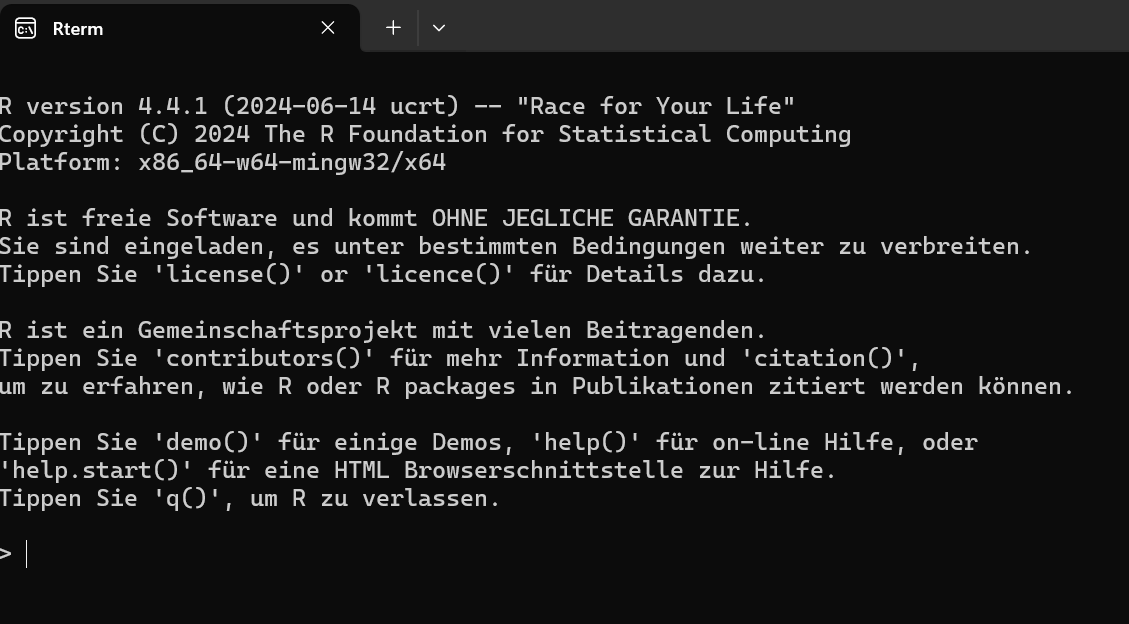
\includegraphics[width=0.65\linewidth,height=\textheight,keepaspectratio]{../figures/R_Konsole.png}
\end{frame}

\begin{frame}[fragile]{Die R-Konsole}
\phantomsection\label{die-r-konsole}
Eingabe

\begin{Shaded}
\begin{Highlighting}[]
\DecValTok{1} \SpecialCharTok{+} \DecValTok{2}
\end{Highlighting}
\end{Shaded}

Ausgabe

\begin{Shaded}
\begin{Highlighting}[]
\NormalTok{[1] 3}
\end{Highlighting}
\end{Shaded}

Nützliche Funktion: alte Befehle mit Pfeiltasten abrufen
\end{frame}

\begin{frame}[fragile]{Skripte in R}
\phantomsection\label{skripte-in-r}
Warum Skripte?

\begin{itemize}
\tightlist
\item
  Code speichern
\item
  erneut ausführen
\item
  dokumentieren
\item
  reproduzierbar arbeiten
\end{itemize}

Dateiendung

\begin{Shaded}
\begin{Highlighting}[]
\NormalTok{.R}
\end{Highlighting}
\end{Shaded}
\end{frame}

\begin{frame}{Konsole vs.~Skript}
\phantomsection\label{konsole-vs.-skript}
\begin{longtable}[]{@{}ll@{}}
\toprule\noalign{}
Konsole & Skript \\
\midrule\noalign{}
\endhead
schnelle Tests & strukturierter Code \\
temporär & dauerhaft speicherbar \\
einzelne Befehle & komplette Analysen \\
\bottomrule\noalign{}
\end{longtable}
\end{frame}

\begin{frame}{RStudio Oberfläche}
\phantomsection\label{rstudio-oberfluxe4che}
\begin{figure}[H]

{\centering \pandocbounded{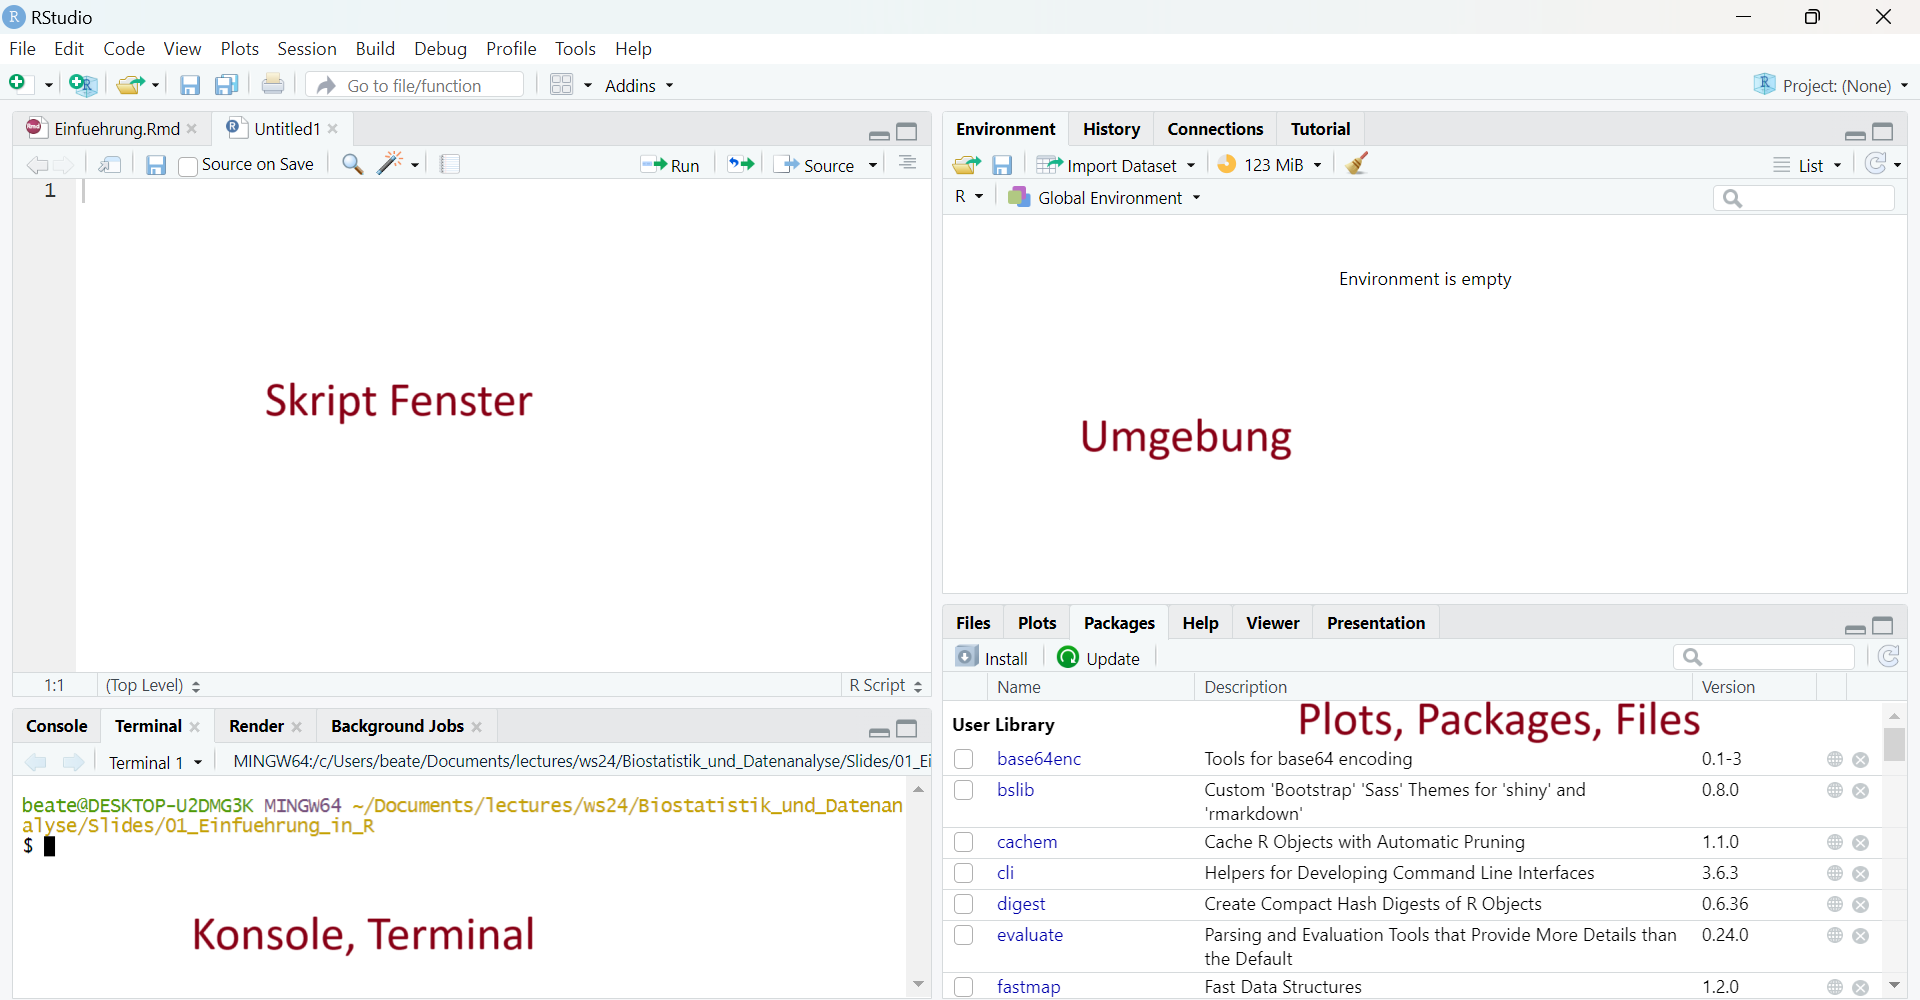
\includegraphics[keepaspectratio]{../figures/RStudio.png}}

}

\caption{RStudio Oberfläche}

\end{figure}%
\end{frame}

\begin{frame}[fragile]{Neues Skript erstellen}
\phantomsection\label{neues-skript-erstellen}
Menü

\begin{Shaded}
\begin{Highlighting}[]
\NormalTok{File \textgreater{} New File \textgreater{} R Script}
\end{Highlighting}
\end{Shaded}
\end{frame}

\begin{frame}[fragile]{Erstes Programm}
\phantomsection\label{erstes-programm}
\begin{Shaded}
\begin{Highlighting}[]
\FunctionTok{print}\NormalTok{(}\StringTok{"Hello, world"}\NormalTok{)}
\end{Highlighting}
\end{Shaded}
\end{frame}

\begin{frame}[fragile]{Programm ausführen}
\phantomsection\label{programm-ausfuxfchren}
Tastenkombination

\begin{Shaded}
\begin{Highlighting}[]
\NormalTok{Strg + Enter}
\end{Highlighting}
\end{Shaded}

Alternative: Button „Run``
\end{frame}

\begin{frame}{Beispiel: Hello World}
\phantomsection\label{beispiel-hello-world}
\pandocbounded{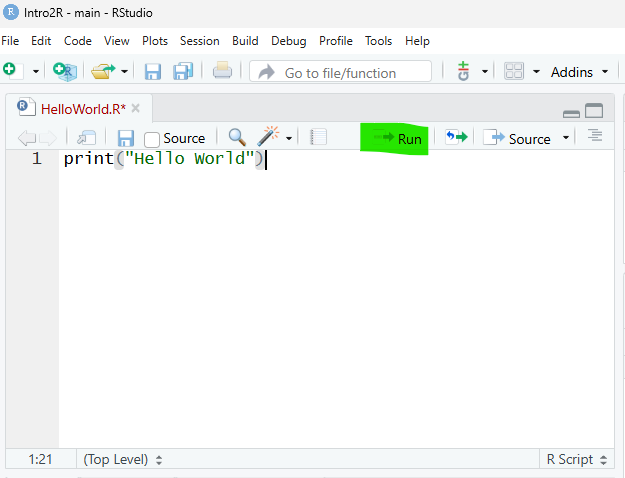
\includegraphics[keepaspectratio]{../figures/Skript.png}}
\end{frame}

\begin{frame}[fragile]{Funktionen in R}
\phantomsection\label{funktionen-in-r}
Allgemeine Struktur

\begin{Shaded}
\begin{Highlighting}[]
\FunctionTok{funktionsname}\NormalTok{(argumente)}
\end{Highlighting}
\end{Shaded}

Beispiel

\begin{Shaded}
\begin{Highlighting}[]
\FunctionTok{print}\NormalTok{(}\StringTok{"Hello, world"}\NormalTok{)}
\end{Highlighting}
\end{Shaded}
\end{frame}

\begin{frame}[fragile]{Funktionen und Argumente}
\phantomsection\label{funktionen-und-argumente}
\begin{Shaded}
\begin{Highlighting}[]
\FunctionTok{print}\NormalTok{(}\StringTok{"Hello, world"}\NormalTok{)}
\end{Highlighting}
\end{Shaded}

\begin{itemize}
\tightlist
\item
  \texttt{print()} ist die Funktion
\item
  \texttt{"Hello,\ world"} ist das Argument
\end{itemize}
\end{frame}

\begin{frame}{Zusatzpakete}
\phantomsection\label{zusatzpakete}
Pakete enthalten zusätzlichen Code für:

\begin{itemize}
\tightlist
\item
  Statistik
\item
  Datenanalyse
\item
  Visualisierung
\item
  Machine Learning
\end{itemize}
\end{frame}

\begin{frame}[fragile]{Pakete installieren}
\phantomsection\label{pakete-installieren}
\begin{Shaded}
\begin{Highlighting}[]
\FunctionTok{install.packages}\NormalTok{(}\StringTok{"dplyr"}\NormalTok{)}
\end{Highlighting}
\end{Shaded}
\end{frame}

\begin{frame}[fragile]{Installation mit Abhängigkeiten}
\phantomsection\label{installation-mit-abhuxe4ngigkeiten}
\begin{Shaded}
\begin{Highlighting}[]
\FunctionTok{install.packages}\NormalTok{(}
  \StringTok{"dplyr"}\NormalTok{,}
  \AttributeTok{dependencies =} \ConstantTok{TRUE}
\NormalTok{)}
\end{Highlighting}
\end{Shaded}

Vorteil: notwendige Zusatzpakete werden automatisch installiert
\end{frame}

\begin{frame}[fragile]{R als Taschenrechner}
\phantomsection\label{r-als-taschenrechner}
Grundrechenarten

\begin{itemize}
\tightlist
\item
  Addition \texttt{+}
\item
  Subtraktion \texttt{-}
\item
  Multiplikation \texttt{*}
\item
  Division \texttt{/}
\item
  Potenzen \texttt{\^{}}
\end{itemize}
\end{frame}

\begin{frame}[fragile]{Kommentare in R}
\phantomsection\label{kommentare-in-r}
\begin{Shaded}
\begin{Highlighting}[]
\DecValTok{5} \SpecialCharTok{{-}} \DecValTok{1}\SpecialCharTok{/}\DecValTok{2}  \CommentTok{\# Kommentar}
\end{Highlighting}
\end{Shaded}

Kommentare beginnen mit

\begin{Shaded}
\begin{Highlighting}[]
\CommentTok{\#}
\end{Highlighting}
\end{Shaded}
\end{frame}

\begin{frame}{Kommentare sind wichtig}
\phantomsection\label{kommentare-sind-wichtig}
\begin{itemize}
\tightlist
\item
  bessere Lesbarkeit
\item
  Dokumentation
\item
  Zusammenarbeit erleichtern
\item
  spätere Nachvollziehbarkeit
\end{itemize}
\end{frame}

\begin{frame}[fragile]{Arithmetische Ausdrücke}
\phantomsection\label{arithmetische-ausdruxfccke}
\begin{Shaded}
\begin{Highlighting}[]
\NormalTok{(}\DecValTok{1} \SpecialCharTok{+} \DecValTok{2}\NormalTok{) }\SpecialCharTok{/}\NormalTok{ (}\DecValTok{4} \SpecialCharTok{{-}} \FloatTok{1.2}\NormalTok{) }\SpecialCharTok{*} \DecValTok{2}\SpecialCharTok{\^{}}\DecValTok{10}
\end{Highlighting}
\end{Shaded}
\end{frame}

\begin{frame}[fragile]{Operatoren}
\phantomsection\label{operatoren}
\begin{longtable}[]{@{}ll@{}}
\toprule\noalign{}
Operator & Bedeutung \\
\midrule\noalign{}
\endhead
\texttt{+} & Addition \\
\texttt{-} & Subtraktion \\
\texttt{*} & Multiplikation \\
\texttt{/} & Division \\
\texttt{\^{}} & Potenz \\
\bottomrule\noalign{}
\end{longtable}
\end{frame}

\begin{frame}{Berechnen Sie}
\phantomsection\label{berechnen-sie}
\begin{itemize}
\tightlist
\item
  \(2^8\)
\item
  den Umfang eines Kreises mit \(r=2\)
\item
  \(log_{10}(1000)\)
\item
  Runden Sie \(\pi\) auf 4 Nachkommastellen
\item
  \(\frac{\sqrt{25} + 3^2}{log_2(8)}\)
\end{itemize}
\end{frame}

\begin{frame}[fragile]{Achtung: \texttt{log()}}
\phantomsection\label{achtung-log}
\begin{Shaded}
\begin{Highlighting}[]
\FunctionTok{log}\NormalTok{(x)}
\end{Highlighting}
\end{Shaded}

berechnet den natürlichen Logarithmus.

Logarithmus zur Basis 10

\begin{Shaded}
\begin{Highlighting}[]
\FunctionTok{log10}\NormalTok{(x)}
\end{Highlighting}
\end{Shaded}
\end{frame}

\begin{frame}[fragile]{Prioritäten von Operatoren}
\phantomsection\label{priorituxe4ten-von-operatoren}
Punkt vor Strich

\begin{Shaded}
\begin{Highlighting}[]
\DecValTok{1} \SpecialCharTok{+} \DecValTok{2} \SpecialCharTok{*} \DecValTok{3}
\end{Highlighting}
\end{Shaded}

entspricht:

\begin{Shaded}
\begin{Highlighting}[]
\DecValTok{1} \SpecialCharTok{+}\NormalTok{ (}\DecValTok{2} \SpecialCharTok{*} \DecValTok{3}\NormalTok{)}
\end{Highlighting}
\end{Shaded}

Klammern ändern die Reihenfolge

\begin{Shaded}
\begin{Highlighting}[]
\NormalTok{(}\DecValTok{1} \SpecialCharTok{+} \DecValTok{2}\NormalTok{) }\SpecialCharTok{*} \DecValTok{3}
\end{Highlighting}
\end{Shaded}
\end{frame}

\begin{frame}[fragile]{Operatoren und Operanden}
\phantomsection\label{operatoren-und-operanden}
Operatoren verknüpfen oder verändern \textbf{Operanden}.

\begin{itemize}
\tightlist
\item
  Operanden = Werte oder Ausdrücke
\item
  Operatoren = Rechen- oder Vergleichszeichen
\end{itemize}

Beispiele:

\begin{Shaded}
\begin{Highlighting}[]
\DecValTok{2} \SpecialCharTok{+} \DecValTok{3}
\DecValTok{5} \SpecialCharTok{*} \DecValTok{8}
\NormalTok{x }\OtherTok{\textless{}{-}} \DecValTok{4}
\end{Highlighting}
\end{Shaded}
\end{frame}

\begin{frame}[fragile]{Binäre Operatoren}
\phantomsection\label{binuxe4re-operatoren}
Binäre Operatoren arbeiten mit \textbf{zwei Argumenten}.

\begin{longtable}[]{@{}ll@{}}
\toprule\noalign{}
Operator & Bedeutung \\
\midrule\noalign{}
\endhead
\texttt{+} & Addition \\
\texttt{-} & Subtraktion \\
\texttt{*} & Multiplikation \\
\texttt{/} & Division \\
\texttt{\^{}} & Potenz \\
\texttt{\textless{}-} & Zuweisung \\
\bottomrule\noalign{}
\end{longtable}
\end{frame}

\begin{frame}[fragile]{Linksassoziative Operatoren}
\phantomsection\label{linksassoziative-operatoren}
Auswertung von links nach rechts

Beispiel

\begin{Shaded}
\begin{Highlighting}[]
\DecValTok{1} \SpecialCharTok{/} \DecValTok{2} \SpecialCharTok{/} \DecValTok{3}
\end{Highlighting}
\end{Shaded}

R interpretiert dies als: \(\left(\frac{1}{2}\right)/3\)
\end{frame}

\begin{frame}[fragile]{Rechtsassoziative Operatoren}
\phantomsection\label{rechtsassoziative-operatoren}
Potenzoperator \texttt{\^{}}: wird von rechts nach links ausgewertet

Beispiel

\begin{Shaded}
\begin{Highlighting}[]
\DecValTok{2}\SpecialCharTok{\^{}}\DecValTok{3}\SpecialCharTok{\^{}}\DecValTok{4}
\end{Highlighting}
\end{Shaded}

Interpretation: \(2^{(3^4)}\)

Nicht: \((2^3)^4\)
\end{frame}

\begin{frame}[fragile]{Unäre Operatoren}
\phantomsection\label{unuxe4re-operatoren}
Ein Argument: Unäre Operatoren arbeiten mit genau einem Operanden.

Beispiel: Negation

\begin{Shaded}
\begin{Highlighting}[]
\SpecialCharTok{!}\ConstantTok{TRUE}
\end{Highlighting}
\end{Shaded}

Ergebnis:

\begin{Shaded}
\begin{Highlighting}[]
\ConstantTok{FALSE}
\end{Highlighting}
\end{Shaded}
\end{frame}

\begin{frame}[fragile]{Operatoren als Funktionen}
\phantomsection\label{operatoren-als-funktionen}
In R sind Operatoren intern Funktionen.

\begin{Shaded}
\begin{Highlighting}[]
\DecValTok{7} \SpecialCharTok{+} \DecValTok{3}
\end{Highlighting}
\end{Shaded}

ist identisch zu:

\begin{Shaded}
\begin{Highlighting}[]
\StringTok{\textasciigrave{}}\AttributeTok{+}\StringTok{\textasciigrave{}}\NormalTok{(}\DecValTok{7}\NormalTok{, }\DecValTok{3}\NormalTok{)}
\end{Highlighting}
\end{Shaded}

Vergleich:

\begin{Shaded}
\begin{Highlighting}[]
\DecValTok{7} \SpecialCharTok{+} \DecValTok{3} \SpecialCharTok{==} \StringTok{\textasciigrave{}}\AttributeTok{+}\StringTok{\textasciigrave{}}\NormalTok{(}\DecValTok{7}\NormalTok{, }\DecValTok{3}\NormalTok{)}
\end{Highlighting}
\end{Shaded}
\end{frame}

\begin{frame}[fragile]{Arithmetische Operatoren}
\phantomsection\label{arithmetische-operatoren}
\begin{longtable}[]{@{}ll@{}}
\toprule\noalign{}
Operator & Bedeutung \\
\midrule\noalign{}
\endhead
\texttt{+} & Addition \\
\texttt{-} & Subtraktion \\
\texttt{*} & Multiplikation \\
\texttt{/} & Division \\
\texttt{\^{}} & Potenz \\
\texttt{\%/\%} & Ganzzahlige Division \\
\texttt{\%\%} & Modulo \\
\bottomrule\noalign{}
\end{longtable}

Beispiele

\begin{Shaded}
\begin{Highlighting}[]
\DecValTok{5} \SpecialCharTok{\%/\%} \DecValTok{2}
\DecValTok{5} \SpecialCharTok{\%\%} \DecValTok{2}
\end{Highlighting}
\end{Shaded}
\end{frame}

\begin{frame}[fragile]{Logische Operatoren}
\phantomsection\label{logische-operatoren}
Vergleichsoperatoren

\begin{longtable}[]{@{}ll@{}}
\toprule\noalign{}
Operator & Bedeutung \\
\midrule\noalign{}
\endhead
\texttt{\textless{}} & kleiner \\
\texttt{\textless{}=} & kleiner gleich \\
\texttt{\textgreater{}} & größer \\
\texttt{\textgreater{}=} & größer gleich \\
\texttt{==} & gleich \\
\texttt{!=} & ungleich \\
\bottomrule\noalign{}
\end{longtable}
\end{frame}

\begin{frame}[fragile]{Logische Verknüpfungen}
\phantomsection\label{logische-verknuxfcpfungen}
Wahrheitswerte kombinieren

\begin{longtable}[]{@{}ll@{}}
\toprule\noalign{}
Operator & Bedeutung \\
\midrule\noalign{}
\endhead
\texttt{!x} & NICHT \\
\texttt{x\ \&\ y} & UND \\
\texttt{x\ \textbar{}\ y} & ODER \\
\bottomrule\noalign{}
\end{longtable}

Beispiel

\begin{Shaded}
\begin{Highlighting}[]
\ConstantTok{TRUE} \SpecialCharTok{\&} \ConstantTok{FALSE}
\ConstantTok{TRUE} \SpecialCharTok{|} \ConstantTok{FALSE}
\SpecialCharTok{!}\ConstantTok{TRUE}
\end{Highlighting}
\end{Shaded}
\end{frame}

\begin{frame}[fragile]{Aufgabe}
\phantomsection\label{aufgabe}
Definieren Sie folgende Variablen:

\begin{Shaded}
\begin{Highlighting}[]
\NormalTok{itsRaining }\OtherTok{\textless{}{-}} \ConstantTok{TRUE}
\NormalTok{haveUmbrella }\OtherTok{\textless{}{-}} \ConstantTok{FALSE}
\end{Highlighting}
\end{Shaded}

Berechnen Sie anschließend:

\begin{enumerate}
\tightlist
\item
  Regnet es \textbf{und} haben Sie einen Regenschirm?
\item
  Regnet es \textbf{oder} haben Sie einen Regenschirm?
\item
  Bleiben Sie trocken, wenn Sie einen Regenschirm haben oder es nicht
  regnet?
\end{enumerate}
\end{frame}

\begin{frame}[fragile]{Arbeiten mit Vektoren}
\phantomsection\label{arbeiten-mit-vektoren}
Vektoren werden mit \texttt{c()} erstellt.

Beispiel

\begin{Shaded}
\begin{Highlighting}[]
\NormalTok{x }\OtherTok{\textless{}{-}} \FunctionTok{c}\NormalTok{(}\DecValTok{1}\NormalTok{, }\DecValTok{2}\NormalTok{, }\DecValTok{5}\NormalTok{, }\DecValTok{7}\NormalTok{)}
\end{Highlighting}
\end{Shaded}

Ausgabe:

\begin{Shaded}
\begin{Highlighting}[]
\NormalTok{x}
\end{Highlighting}
\end{Shaded}
\end{frame}

\begin{frame}[fragile]{Mittelwert berechnen}
\phantomsection\label{mittelwert-berechnen}
Funktion \texttt{mean()}

\begin{Shaded}
\begin{Highlighting}[]
\NormalTok{x }\OtherTok{\textless{}{-}} \FunctionTok{c}\NormalTok{(}\DecValTok{1}\NormalTok{, }\DecValTok{2}\NormalTok{, }\DecValTok{5}\NormalTok{, }\DecValTok{7}\NormalTok{)}

\FunctionTok{mean}\NormalTok{(x)}
\end{Highlighting}
\end{Shaded}
\end{frame}

\begin{frame}[fragile]{Standardabweichung}
\phantomsection\label{standardabweichung}
Funktion \texttt{sd()}

\begin{Shaded}
\begin{Highlighting}[]
\NormalTok{x }\OtherTok{\textless{}{-}} \FunctionTok{c}\NormalTok{(}\DecValTok{1}\NormalTok{, }\DecValTok{2}\NormalTok{, }\DecValTok{5}\NormalTok{, }\DecValTok{7}\NormalTok{)}

\FunctionTok{sd}\NormalTok{(x)}
\end{Highlighting}
\end{Shaded}
\end{frame}

\begin{frame}[fragile]{Runden mit \texttt{round()}}
\phantomsection\label{runden-mit-round}
Ganze Zahlen

\begin{Shaded}
\begin{Highlighting}[]
\FunctionTok{round}\NormalTok{(}\DecValTok{7}\SpecialCharTok{/}\DecValTok{3}\NormalTok{)}
\end{Highlighting}
\end{Shaded}

Mit Nachkommastellen

\begin{Shaded}
\begin{Highlighting}[]
\FunctionTok{round}\NormalTok{(}\DecValTok{7}\SpecialCharTok{/}\DecValTok{3}\NormalTok{, }\AttributeTok{digits =} \DecValTok{3}\NormalTok{)}
\end{Highlighting}
\end{Shaded}
\end{frame}

\begin{frame}[fragile]{Potenzen in R}
\phantomsection\label{potenzen-in-r}
Potenzoperator \texttt{\^{}}

\begin{Shaded}
\begin{Highlighting}[]
\DecValTok{10}\SpecialCharTok{\^{}}\DecValTok{5}
\end{Highlighting}
\end{Shaded}
\end{frame}

\begin{frame}[fragile]{Wissenschaftliche Notation}
\phantomsection\label{wissenschaftliche-notation}
Große und kleine Zahlen

\[
100000 = 1 \times 10^5
\]

\[
0.0012 = 1.2 \times 10^{-3}
\]

Beispiel in R

\begin{Shaded}
\begin{Highlighting}[]
\NormalTok{x }\OtherTok{\textless{}{-}} \DecValTok{1} \SpecialCharTok{*} \DecValTok{10}\SpecialCharTok{\^{}}\DecValTok{5}
\end{Highlighting}
\end{Shaded}
\end{frame}

\begin{frame}[fragile]{Logarithmus Basis 10}
\phantomsection\label{logarithmus-basis-10}
Funktion \texttt{log10()}

\begin{Shaded}
\begin{Highlighting}[]
\DecValTok{10}\SpecialCharTok{\^{}}\DecValTok{6}
\end{Highlighting}
\end{Shaded}

\begin{Shaded}
\begin{Highlighting}[]
\FunctionTok{log10}\NormalTok{(}\FloatTok{1e6}\NormalTok{)}
\end{Highlighting}
\end{Shaded}
\end{frame}

\begin{frame}[fragile]{Logarithmus Basis 2}
\phantomsection\label{logarithmus-basis-2}
Funktion \texttt{log2()}

\begin{Shaded}
\begin{Highlighting}[]
\DecValTok{2}\SpecialCharTok{\^{}}\DecValTok{10}
\end{Highlighting}
\end{Shaded}

\begin{Shaded}
\begin{Highlighting}[]
\FunctionTok{log2}\NormalTok{(}\DecValTok{1024}\NormalTok{)}
\end{Highlighting}
\end{Shaded}
\end{frame}

\begin{frame}[fragile]{Natürlicher Logarithmus}
\phantomsection\label{natuxfcrlicher-logarithmus}
Basis (e)

\begin{Shaded}
\begin{Highlighting}[]
\FunctionTok{exp}\NormalTok{(}\DecValTok{1}\NormalTok{)}
\end{Highlighting}
\end{Shaded}

\begin{Shaded}
\begin{Highlighting}[]
\FunctionTok{log}\NormalTok{(}\FunctionTok{exp}\NormalTok{(}\DecValTok{1}\NormalTok{))}
\end{Highlighting}
\end{Shaded}
\end{frame}

\begin{frame}[fragile]{Hilfe in R}
\phantomsection\label{hilfe-in-r}
Hilfe aufrufen

\begin{Shaded}
\begin{Highlighting}[]
\NormalTok{?mean}
\end{Highlighting}
\end{Shaded}

Alternative

\begin{Shaded}
\begin{Highlighting}[]
\FunctionTok{help}\NormalTok{(}\StringTok{"mean"}\NormalTok{)}
\end{Highlighting}
\end{Shaded}

Suche

\begin{Shaded}
\begin{Highlighting}[]
\FunctionTok{help.search}\NormalTok{(}\StringTok{"mean"}\NormalTok{)}
\end{Highlighting}
\end{Shaded}
\end{frame}

\begin{frame}{Alles ist ein Objekt}
\phantomsection\label{alles-ist-ein-objekt}
\begin{quote}
Everything that exists is an object.\\
Everything that happens is a function call.
\end{quote}

--- John Chambers
\end{frame}

\begin{frame}[fragile]{Funktionen in R}
\phantomsection\label{funktionen-in-r-1}
Funktionen verarbeiten Input

\begin{block}{Beispiel}
\phantomsection\label{beispiel}
\begin{Shaded}
\begin{Highlighting}[]
\DecValTok{2} \SpecialCharTok{+} \DecValTok{3}
\end{Highlighting}
\end{Shaded}

Ergebnis:

\begin{Shaded}
\begin{Highlighting}[]
\DecValTok{5}
\end{Highlighting}
\end{Shaded}
\end{block}
\end{frame}

\begin{frame}[fragile]{Variablen und Zuweisungen}
\phantomsection\label{variablen-und-zuweisungen}
Mit \texttt{\textless{}-}

\begin{Shaded}
\begin{Highlighting}[]
\NormalTok{x }\OtherTok{\textless{}{-}} \DecValTok{2}
\NormalTok{y }\OtherTok{\textless{}{-}} \DecValTok{3}
\NormalTok{z }\OtherTok{\textless{}{-}}\NormalTok{ x }\SpecialCharTok{+}\NormalTok{ y}
\end{Highlighting}
\end{Shaded}
\end{frame}

\begin{frame}{Warum \texttt{\textless{}-}?}
\phantomsection\label{warum--}
\begin{itemize}
\tightlist
\item
  Richtung der Zuweisung sichtbar
\item
  Historisch aus der Sprache S übernommen
\item
  Bessere Lesbarkeit
\end{itemize}
\end{frame}

\begin{frame}[fragile]{Variablennamen}
\phantomsection\label{variablennamen}
Regeln

Erlaubt:

\begin{itemize}
\tightlist
\item
  Buchstaben
\item
  Zahlen
\item
  \texttt{\_}
\item
  \texttt{.}
\end{itemize}

Nicht erlaubt:

\begin{itemize}
\tightlist
\item
  Beginn mit Zahl
\item
  reservierte Wörter
\end{itemize}
\end{frame}

\begin{frame}[fragile]{Gültige Namen}
\phantomsection\label{guxfcltige-namen}
Beispiele

\begin{Shaded}
\begin{Highlighting}[]
\NormalTok{x1}
\NormalTok{X1}
\NormalTok{min.dist}
\NormalTok{Best.gene}
\end{Highlighting}
\end{Shaded}
\end{frame}

\begin{frame}[fragile]{Ungültige Namen}
\phantomsection\label{unguxfcltige-namen}
Beispiel

\begin{Shaded}
\begin{Highlighting}[]
\ConstantTok{TRUE} \OtherTok{\textless{}{-}} \DecValTok{5}
\end{Highlighting}
\end{Shaded}

Fehler:

\begin{Shaded}
\begin{Highlighting}[]
\NormalTok{Error }\ControlFlowTok{in} \ConstantTok{TRUE} \OtherTok{\textless{}{-}} \DecValTok{5}
\end{Highlighting}
\end{Shaded}
\end{frame}

\begin{frame}[fragile]{Funktionen als Blackbox}
\phantomsection\label{funktionen-als-blackbox}
Input → Verarbeitung → Output

\begin{block}{Beispiel}
\phantomsection\label{beispiel-1}
\begin{Shaded}
\begin{Highlighting}[]
\FunctionTok{mean}\NormalTok{(}\FunctionTok{c}\NormalTok{(}\DecValTok{1}\NormalTok{,}\DecValTok{2}\NormalTok{,}\DecValTok{3}\NormalTok{))}
\end{Highlighting}
\end{Shaded}
\end{block}
\end{frame}

\begin{frame}[fragile]{Parameter in Funktionen}
\phantomsection\label{parameter-in-funktionen}
Standardwerte

\begin{Shaded}
\begin{Highlighting}[]
\NormalTok{x }\OtherTok{\textless{}{-}} \FunctionTok{c}\NormalTok{(}\DecValTok{1}\NormalTok{, }\ConstantTok{NA}\NormalTok{, }\DecValTok{6}\NormalTok{)}

\FunctionTok{mean}\NormalTok{(x, }\AttributeTok{na.rm =} \ConstantTok{TRUE}\NormalTok{)}
\end{Highlighting}
\end{Shaded}
\end{frame}

\begin{frame}[fragile]{Wichtige Basisfunktionen}
\phantomsection\label{wichtige-basisfunktionen}
\begin{longtable}[]{@{}ll@{}}
\toprule\noalign{}
Funktion & Bedeutung \\
\midrule\noalign{}
\endhead
\texttt{sqrt()} & Wurzel \\
\texttt{abs()} & Absolutwert \\
\texttt{sum()} & Summe \\
\texttt{mean()} & Mittelwert \\
\texttt{max()} & Maximum \\
\bottomrule\noalign{}
\end{longtable}
\end{frame}

\begin{frame}[fragile]{Eigene Funktionen}
\phantomsection\label{eigene-funktionen}
Funktion definieren

\begin{Shaded}
\begin{Highlighting}[]
\NormalTok{pythagoras }\OtherTok{\textless{}{-}} \ControlFlowTok{function}\NormalTok{(a, b)\{}

\NormalTok{  hypo }\OtherTok{\textless{}{-}} \FunctionTok{sqrt}\NormalTok{(a}\SpecialCharTok{\^{}}\DecValTok{2} \SpecialCharTok{+}\NormalTok{ b}\SpecialCharTok{\^{}}\DecValTok{2}\NormalTok{)}

  \FunctionTok{return}\NormalTok{(hypo)}
\NormalTok{\}}
\end{Highlighting}
\end{Shaded}

Aufruf:

\begin{Shaded}
\begin{Highlighting}[]
\FunctionTok{pythagoras}\NormalTok{(}\DecValTok{2}\NormalTok{,}\DecValTok{4}\NormalTok{)}
\end{Highlighting}
\end{Shaded}
\end{frame}

\begin{frame}{Satz des Pythagoras}
\phantomsection\label{satz-des-pythagoras}
\[
c = \sqrt{a^2 + b^2}
\]
\end{frame}

\begin{frame}[fragile]{Scope in R}
\phantomsection\label{scope-in-r}
Lokale Variablen

\begin{Shaded}
\begin{Highlighting}[]
\NormalTok{x }\OtherTok{\textless{}{-}} \DecValTok{10}

\NormalTok{demo }\OtherTok{\textless{}{-}} \ControlFlowTok{function}\NormalTok{() \{}
\NormalTok{  x }\OtherTok{\textless{}{-}} \DecValTok{5}
\NormalTok{  x}
\NormalTok{\}}
\end{Highlighting}
\end{Shaded}

Das äußere \texttt{x} bleibt unverändert.
\end{frame}

\begin{frame}[fragile]{Globale Variablen}
\phantomsection\label{globale-variablen}
Zugriff außerhalb von Funktionen

\begin{Shaded}
\begin{Highlighting}[]
\NormalTok{patienten }\OtherTok{\textless{}{-}} \DecValTok{120}
\end{Highlighting}
\end{Shaded}
\end{frame}

\begin{frame}[fragile]{Vorsicht mit \texttt{\textless{}\textless{}-}}
\phantomsection\label{vorsicht-mit--}
Globale Variablen verändern

\begin{Shaded}
\begin{Highlighting}[]
\NormalTok{x }\OtherTok{\textless{}{-}} \DecValTok{1}

\NormalTok{f }\OtherTok{\textless{}{-}} \ControlFlowTok{function}\NormalTok{() \{}
\NormalTok{  x }\OtherTok{\textless{}\textless{}{-}} \DecValTok{99}
\NormalTok{\}}
\end{Highlighting}
\end{Shaded}
\end{frame}

\begin{frame}[fragile]{Einfache Datentypen}
\phantomsection\label{einfache-datentypen}
\begin{longtable}[]{@{}ll@{}}
\toprule\noalign{}
Typ & Bedeutung \\
\midrule\noalign{}
\endhead
\texttt{logical} & Wahr/Falsch \\
\texttt{integer} & Ganze Zahlen \\
\texttt{double} & Fließkommazahlen \\
\texttt{character} & Zeichenketten \\
\bottomrule\noalign{}
\end{longtable}
\end{frame}

\begin{frame}[fragile]{Beispiele Datentypen}
\phantomsection\label{beispiele-datentypen}
\begin{Shaded}
\begin{Highlighting}[]
\NormalTok{iamhappy }\OtherTok{\textless{}{-}} \ConstantTok{TRUE}
\NormalTok{mynumber }\OtherTok{\textless{}{-}} \DecValTok{4}
\NormalTok{n2 }\OtherTok{\textless{}{-}} \FloatTok{0.3}
\NormalTok{hello }\OtherTok{\textless{}{-}} \StringTok{"world"}
\end{Highlighting}
\end{Shaded}
\end{frame}

\begin{frame}[fragile]{Dynamische Typisierung}
\phantomsection\label{dynamische-typisierung}
R erkennt Datentypen automatisch.

\begin{Shaded}
\begin{Highlighting}[]
\NormalTok{x }\OtherTok{\textless{}{-}} \DecValTok{5}
\end{Highlighting}
\end{Shaded}
\end{frame}

\begin{frame}[fragile]{Fließkommazahlen}
\phantomsection\label{flieuxdfkommazahlen}
Rundungsfehler

\begin{Shaded}
\begin{Highlighting}[]
\FunctionTok{sqrt}\NormalTok{(}\DecValTok{2}\NormalTok{)}
\end{Highlighting}
\end{Shaded}

\begin{Shaded}
\begin{Highlighting}[]
\FunctionTok{sqrt}\NormalTok{(}\DecValTok{2}\NormalTok{)}\SpecialCharTok{\^{}}\DecValTok{2}
\end{Highlighting}
\end{Shaded}
\end{frame}

\begin{frame}[fragile]{Vergleich von Fließkommazahlen}
\phantomsection\label{vergleich-von-flieuxdfkommazahlen}
Nicht direkt mit \texttt{==}

\begin{Shaded}
\begin{Highlighting}[]
\NormalTok{x }\OtherTok{\textless{}{-}} \FloatTok{1.1} \SpecialCharTok{{-}} \FloatTok{0.2}
\NormalTok{y }\OtherTok{\textless{}{-}} \FloatTok{0.9}

\FunctionTok{abs}\NormalTok{(x }\SpecialCharTok{{-}}\NormalTok{ y) }\SpecialCharTok{\textless{}} \FloatTok{0.0000001}
\end{Highlighting}
\end{Shaded}
\end{frame}

\begin{frame}[fragile]{Besondere Konstanten}
\phantomsection\label{besondere-konstanten}
Wichtige Spezialwerte

\begin{longtable}[]{@{}ll@{}}
\toprule\noalign{}
Wert & Bedeutung \\
\midrule\noalign{}
\endhead
\texttt{NA} & Fehlender Wert \\
\texttt{Inf} & Unendlich \\
\texttt{NaN} & Not a Number \\
\bottomrule\noalign{}
\end{longtable}
\end{frame}

\begin{frame}[fragile]{Logische Werte}
\phantomsection\label{logische-werte}
Bedingungen formulieren

\begin{Shaded}
\begin{Highlighting}[]
\NormalTok{itsRaining }\OtherTok{\textless{}{-}} \ConstantTok{TRUE}
\NormalTok{SprinklerOn }\OtherTok{\textless{}{-}} \ConstantTok{FALSE}

\NormalTok{itsRaining }\SpecialCharTok{|}\NormalTok{ SprinklerOn}
\end{Highlighting}
\end{Shaded}
\end{frame}

\begin{frame}[fragile]{Funktionen für logische Vektoren}
\phantomsection\label{funktionen-fuxfcr-logische-vektoren}
\texttt{all()} und \texttt{any()}

\begin{Shaded}
\begin{Highlighting}[]
\FunctionTok{all}\NormalTok{(}\FunctionTok{c}\NormalTok{(}\ConstantTok{TRUE}\NormalTok{, }\ConstantTok{TRUE}\NormalTok{))}
\end{Highlighting}
\end{Shaded}

\begin{Shaded}
\begin{Highlighting}[]
\FunctionTok{any}\NormalTok{(}\FunctionTok{c}\NormalTok{(}\ConstantTok{FALSE}\NormalTok{, }\ConstantTok{TRUE}\NormalTok{))}
\end{Highlighting}
\end{Shaded}
\end{frame}

\begin{frame}[fragile]{Typische Fehler in R}
\phantomsection\label{typische-fehler-in-r}
\begin{itemize}
\tightlist
\item
  \texttt{=} statt \texttt{==}
\item
  Direkter Vergleich von Fließkommazahlen
\item
  Fehlende Werte (\texttt{NA})
\item
  Vergleich logischer Vektoren
\end{itemize}
\end{frame}

\begin{frame}[fragile]{Datentypen prüfen}
\phantomsection\label{datentypen-pruxfcfen}
\begin{Shaded}
\begin{Highlighting}[]
\FunctionTok{is.na}\NormalTok{(x)}
\FunctionTok{is.numeric}\NormalTok{(x)}
\FunctionTok{as.integer}\NormalTok{(x)}
\end{Highlighting}
\end{Shaded}
\end{frame}

\begin{frame}
\end{frame}




\end{document}
